\chapter{Duyệt và phát hành}
\label{chuong:duyet}

Đề chỉ tới học sinh sau hai bước của thầy cô: \textbf{duyệt} (thầy cô đã đọc và ưng), rồi \textbf{phát
hành} cho lớp với giờ mở, giờ đóng. Kriky không tự làm hai bước này.

Hình~\ref{fig:trang-thai-de} là các trạng thái một đề đi qua. Thầy cô thấy đúng những chữ này ở cột
\nhan{TRẠNG THÁI} của \nhan{Các bài kiểm tra}.

\begin{figure}[htbp]
  \centering
  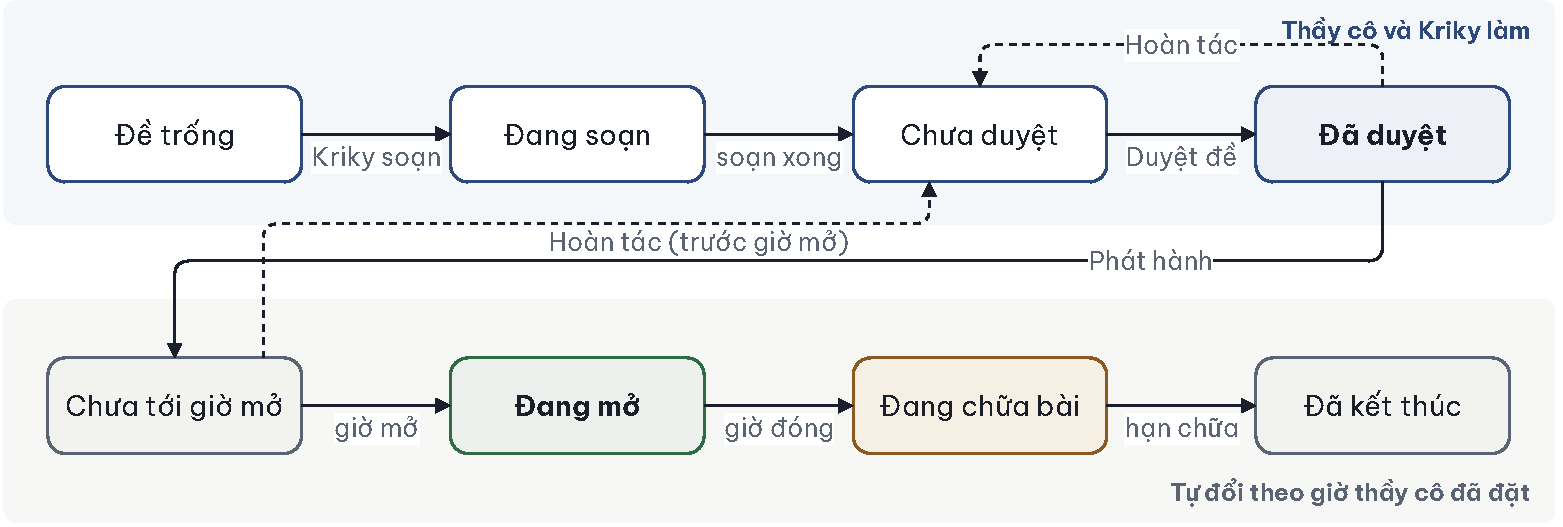
\includegraphics[width=\linewidth]{trang-thai-de.pdf}
  \caption[Trạng thái của một đề]{Trạng thái của một đề. Hàng trên do thầy cô và Kriky làm; hàng dưới
    tự đổi theo giờ thầy cô đã đặt lúc phát hành.}
  \label{fig:trang-thai-de}
\end{figure}

\viec{Duyệt đề}

\anh[0.6\linewidth]{T/19b-duyet-de}{
  \diem{1}{0.2}{0.68}
}

Đọc hết các câu trong khung đề, rồi bấm \nut{Duyệt đề} \sobuoc{1}.

\xong{các câu khoá lại (không còn \nut{Sửa}, \nut{Xoá}), và dưới đề hiện \nhan{Cài đặt phát hành}.}

\machnho{Duyệt đề cũng đưa các câu vào ngân hàng câu hỏi để dùng lại về sau. Duyệt nhầm thì bấm
\nut{Hoàn tác} dưới \nhan{Cài đặt phát hành}: đề về \nhan{Chưa duyệt} và sửa được tiếp.}

\viec{Đặt giờ và phát hành}

\anh[0.62\linewidth]{T/25-cai-dat-phat-hanh}{
  \diem{1}{0.22}{0.145}
  \diem{2}{0.025}{0.32}
  \diem{3}{0.34}{0.32}
  \diem{4}{0.025}{0.42}
  \diem{5}{0.025}{0.6}
  \diem{6}{0.34}{0.6}
  \diem{7}{0.95}{0.65}
  \diem{8}{0.3}{0.93}
}

\begin{buoc}
  \item Bấm lớp sẽ nhận đề (chọn được nhiều lớp).
  \item \nhan{Làm bài}: số phút cho mỗi em làm bài.
  \item \nhan{Mở lúc}: từ giờ này các em bắt đầu làm được.
  \item \nhan{Đóng lúc}: sau giờ này không em nào bắt đầu làm được nữa.
  \item \nhan{Phút mỗi câu}: thời gian cho mỗi câu khi các em làm lại câu sai.
  \item \nhan{Hạn chữa xong}: sau giờ này các em thôi chữa bài.
  \item Đọc khung vàng: Kriky đọc lại các giờ bằng lời để thầy cô kiểm.
  \item Bấm \nut{Phát hành đề}.
\end{buoc}

\begin{bangtra}{L{4.4cm}Y}{\dau{Giờ} & \dau{Cần đúng thế này}}
  \nhan{Mở lúc} & Ở tương lai, sau giờ bấm phát hành. \\
  \nhan{Đóng lúc} & Sau giờ mở. Em vào lúc sát giờ đóng vẫn được làm đủ số phút. \\
  \nhan{Hạn chữa xong} & Sau giờ đóng cộng thời gian làm bài. \\
\end{bangtra}

\viec{Xác nhận phát hành}

\anh[0.62\linewidth]{T/26-xac-nhan-phat-hanh}{
  \diem{1}{0.955}{0.855}
}

Hộp \nhan{Phát hành đề kiểm tra?} đọc lại đề, lớp, giờ và hạn. Đúng hết thì bấm \nut{Phát hành cho 23 học
sinh} \sobuoc{1}. Cần đổi thì bấm \nut{Xem lại cài đặt}.

\xong{khung đề ghi \nhan{ĐÃ PHÁT HÀNH}, thẻ trong chat ghi \nhan{Đã phát hành}.}

\viec{Thu đề về trước giờ mở}

\anh[0.62\linewidth]{T/27-da-phat-hanh}{
  \diem{3}{0.36}{0.9}
}

Phát hành nhầm, hay cần sửa đề, thì thu đề về \textbf{trước giờ mở}:

\begin{buoc}
  \item Mở lại đề: ở \nhan{Các bài kiểm tra} bấm \nut{Mở đoạn chat}, hoặc bấm đoạn chat ấy ở thanh trái
        rồi bấm thẻ đề.
  \item Chỉ thấy dòng \nhan{Cài đặt phát hành} thì bấm vào để mở phần ấy ra.
  \item Bấm \nut{Hoàn tác}.
\end{buoc}

Đề được thu về khỏi mọi lớp và trở lại \nhan{Chưa duyệt}; thầy cô sửa rồi duyệt, phát hành lại.

\luuy{Từ giờ mở, các em đã có thể vào làm, nên không thu đề về được nữa. Chỉ cần một lớp đã tới giờ
mở là \nut{Hoàn tác} khoá. Hoàn tác thu đề khỏi \textbf{mọi} lớp cùng lúc, chưa thu riêng một lớp được.}

\viec{Phát hành thêm cho lớp khác}

Đề đã phát hành vẫn phát thêm được cho lớp chưa nhận: mở khung đề, bấm lớp mới trong \nhan{Cài đặt phát
hành}, đặt giờ, rồi bấm \nut{Phát hành đề}. Lớp đã nhận đề thì chip của nó khoá lại.

\machnho{Ô giờ có thể hiện kiểu 12 giờ, ví dụ \nhan{04:10 CH}: \nhan{CH} là buổi chiều, tức 16:10.}

\machnho{Bỏ dở biểu mẫu giữa chừng thì lần sau mở lại, dòng \nhan{Bản nháp bạn gõ …} giữ các giờ đã gõ.
Bấm \nut{Bỏ bản nháp} để gõ lại từ đầu.}
